
%use mybib.bib for bibliography. bibtex is used for bibliography
\documentclass[journal]{IEEEtran}
\usepackage[utf8]{inputenc}
\usepackage{graphicx}
\usepackage{cite}
\usepackage{longtable}
\usepackage{amsmath}
\usepackage{multirow}
\usepackage{multicol}
%\usepackage{wrapfig}
\usepackage{float}
%\usepackage[section]{placeins}
%\usepackage{subcaption}
\usepackage{array}
\usepackage[export]{adjustbox}
\usepackage{tabu}
\usepackage{listings}
\usepackage{siunitx}
\usepackage{siunitx}
%\usepackage{algorithm}

\usepackage{xcolor}
\colorlet{kw}{blue}
\definecolor{com}{rgb}{0,0.6,0.3}

\usepackage{algorithmicx}
\usepackage{algpseudocode}
\graphicspath{{./figs/}}

%%%%%%%%%%%%%%%%%%%%%%%%%%%%%%%%%%%%%%%%%%%%%%%%%%%%%

% redefine keywords
\algrenewcommand\algorithmicfunction{\textcolor{kw}{function}}
\algrenewcommand\algorithmicwhile{\textcolor{kw}{while}}
\algrenewcommand\algorithmicfor{\textcolor{kw}{for}}
\algrenewcommand\algorithmicif{\textcolor{kw}{if}}
\algrenewcommand\algorithmicelse{\textcolor{kw}{else}}
\algrenewcommand\algorithmicend{\textcolor{kw}{end}}

% new keywords
\algnewcommand\Break{\textcolor{kw}{break}}%
\algnewcommand\Continue{\textcolor{kw}{continue}}%
\algnewcommand\REturn{\textcolor{kw}{return}}%

% redefine loops
\algdef{SE}[WHILE]{While}{EndWhile}[1]{\algorithmicwhile\ #1}{\algorithmicend}%
\algdef{SE}[FOR]{For}{EndFor}[1]{\algorithmicfor\ #1}{\algorithmicend}%
\algdef{C}[IF]{IF}{ElsIf}[1]{\algorithmicelse\algorithmicif\ #1}%

% redefine comments
\algrenewcommand{\algorithmiccomment}[1]{{\color{com}\%#1}}


%%%%%%%%%%%%%%%%%%%%%%%%%%%%%%%%%%%%%%%%%%%%%%%%%%%%%


\ifCLASSINFOpdf

\else

\fi


\hyphenation{op-tical net-works semi-conduc-tor}


\begin{document}

\title{Optimum energy storage control for distributed energy resources based on load, resource availability and real-time price forecasting }

\author{Alvi Newaz, Juan Ospina, Omar Faruque}






\maketitle


\begin{abstract}
Optimizing energy storage management based on present and forecasted data is necessary for efficient operation of distributed energy resources. The purpose of this paper is to present a technique based on A* search algorithm to optimize the use of energy storage. The energy management problem is represented as a graph and A* search algorithm is used to find the optimum actions from the graph to get the minimum cost of operation. A case study has been done using the feeder 2 from the SUNGRIN project \cite{SUNGRIN} and the results are presented.


\end{abstract}



\IEEEpeerreviewmaketitle



\section{Introduction}
In the last few years, there has been significant growth in grid-connected distributed energy resources (DERs) leading to an increased deployment of distributed generation (DG) and recently more distributed storage (DS) systems. Companies are starting to heavily invest in the competitive energy storage system market by taking advantage of the decreasing costs of energy storage. Although a significant amount of DG and DS are being added to the distribution grid, need to improve their control systems for seamless integration to the grid is still there. In the US, most DG and DS systems are deployed to either help reduce the metered load through net-metering programs or to sell power to the utility through power purchase agreements (PPAs). The potential of DG combined with DS is not fully utilized under these pricing schemes due to the lack of proper control. in order to maximize the use of available DERs, a state-of-the-art energy management solution is a necessity for our future electrical grid . Such an energy management solution will be able to dynamically optimize the use of all the available DS with the objective of serving the load in the most economical and safe way possible. This will benefit both utility companies and regular consumers. Due to the constraints and intermittent nature of some DG systems, such as wind and solar, the optimum management of DS combined with a DG is a difficult problem to solve. The most common approaches found in the current literature are as follows. Some researchers formulate the problem as a linear programming (LP) or mixed integer linear programming (MILP) model \cite{lp73, lp74, lp75}. Authors in \cite{pso80, pso81} present an energy management solution based on particle swarm optimization for a microgrid containing wind turbines and energy storage (ES) system. Other researchers propose crow-search and ant colony optimization models to solve the energy management problem for local microgrids as seen in \cite{csa87} and \cite{aco84}. There have also been model predictive control (MPC) based approaches for managing ES in microgrid settings as seen in \cite{energymanajaboulay,mpcmorstyn}.  Researchers in \cite{ga76, ga77} have also proposed genetic algorithm based solutions to optimize the ES operation in a microgrid. One clear disadvantage of these proposed models is that most of these approaches only consider the current status of the system and ignore some critical factors like energy tariff, forecasted load, and forecasted generation profiles.  These information can be used to find an optimum solution based on both current and probable future states of the system as opposed to a solution relying only on the currently available data. Off-line day ahead planning models have also been proposed in the literature. In these methods, available predicted data is used to optimize the scheduling of the ES based on Monte Carlo simulations \cite{6872821,7010943,6839110}. These solutions are very computationally intensive and require a lot of time for planning the day ahead. The computational complexity makes them unsuitable for real-time implementation. Also, as they are off-line calculations they rely vastly on the accuracy of the predictions.

From the discussion thus far, it is evident that there is a need for a real-time ESM solution that can optimize the long-term operating costs of a system containing DG and an energy storage (ES) system. This paper presents an optimum real-time control strategy for such systems. The proposed control strategy takes into account the present and forecasted states of the system, together with the real-time price (RTP), in order to optimize the cost of energy usage. The rest of the paper is organized as follows. Section II discusses how the ESM problem is formulated as a graph search problem. Section III introduces the A* graph search algorithm used to find the optimal solution and how it is used to search for the optimum path of energy decisions. Section IV discusses the test system used in simulation to validate the performance of the graph search based ESM algorithm. Section V discusses the results obtained from the offline simulation and section VI presents the real-time simulation results. Section VII talks about the novelty of the research and section VIII presents the conclusions.

\section{Problem formulation}
The proposed solution technique is designed to be implemented at the point of common coupling (PCC) of a microgrid containing distributed generation (DG) and energy storage (ES). Fig. \ref{fig:system_arch} depicts an example system. Here, the energy storage management system (ESMS) is in charge of controlling the battery connected to the grid with the objective of getting the most cost optimum use of the resources available. The objective of the ESMS is to optimize the use cost of energy storage under different pricing schemes by taking advantage of RTP or time of use (TOU) prices, load and DG generation forecasting.  Fig. \ref{fig:F1_CA} shows the top-level architecture of the ESMS. As seen in the figure, the inputs of the system are the real-time price (RTP) prediction, load prediction, and the DG output prediction, which in this case is a photovoltaic (PV) plant output. It will also consider the current state of the load, current PV generation, and the state of charge of the ES. The output of the ESMS is the optimum battery charge and discharge control references based on the current and forecasted data.

\begin{figure}[!htbp]
\centering
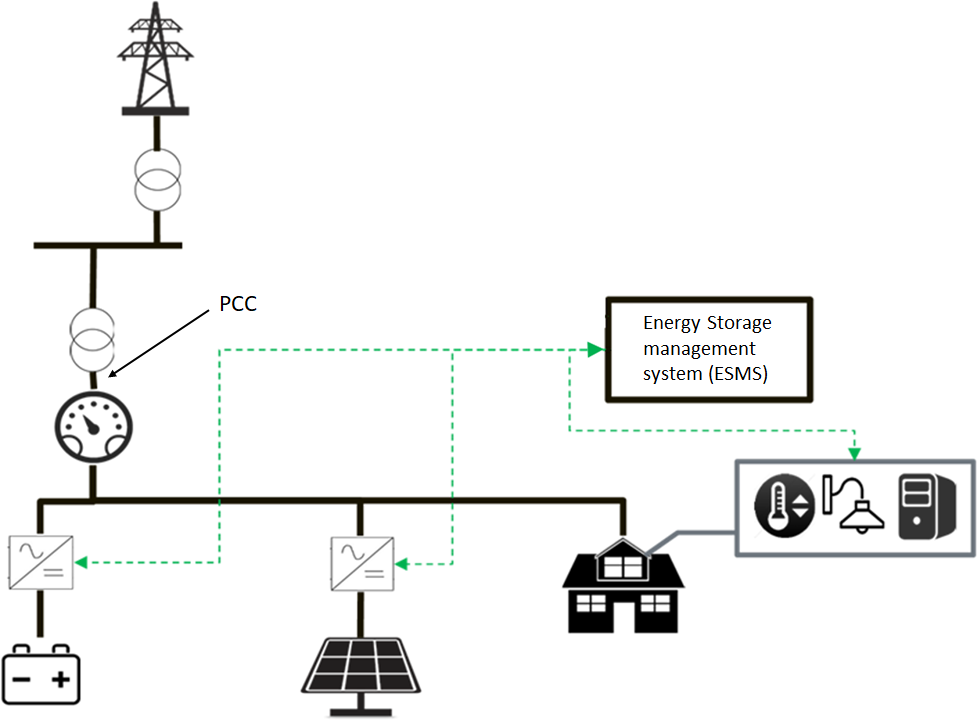
\includegraphics[width=\linewidth]{figs/System_architecture.png}
\caption{Test system architecture}
\label{fig:system_arch}
\vspace{-3mm}
\end{figure}

%  Fig. \ref{fig:F1_CA} shows the top-level architecture of the ESMS. As seen in the figure, the inputs of the system are the real-time price (RTP) prediction, load prediction, and the DG prediction, which in this case is a photovoltaic (PV) plant. It will also consider the current state of the load, PV generation, and ES. The output of the ESMS is the optimum battery charge and discharge control references based on the current and forecasted data.

\begin{figure}[!ht]
    \centering
    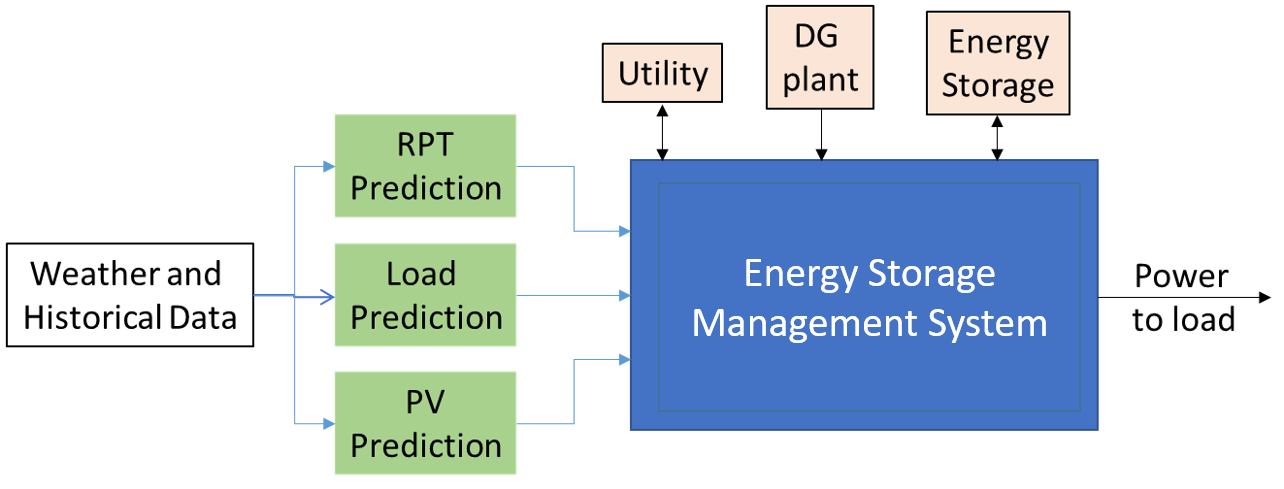
\includegraphics[width = \linewidth]{figs/EMS_FIG.png}
    \caption{Controller top level architecture}
    \label{fig:F1_CA}
\end{figure}

In order to find the optimum cost solution based on the current status of the system and future forecasts, the optimization problem is formulated using a graph search problem approach. To represent the solution space of the problem as a graph, the state of charge (SOC) of the ES, and both the prediction horizon and the control horizon are discretized. Fig. \ref{fig:F1_Dis} demonstrates an example of the discretized solution space.
\begin{figure}[!ht]
    \centering
    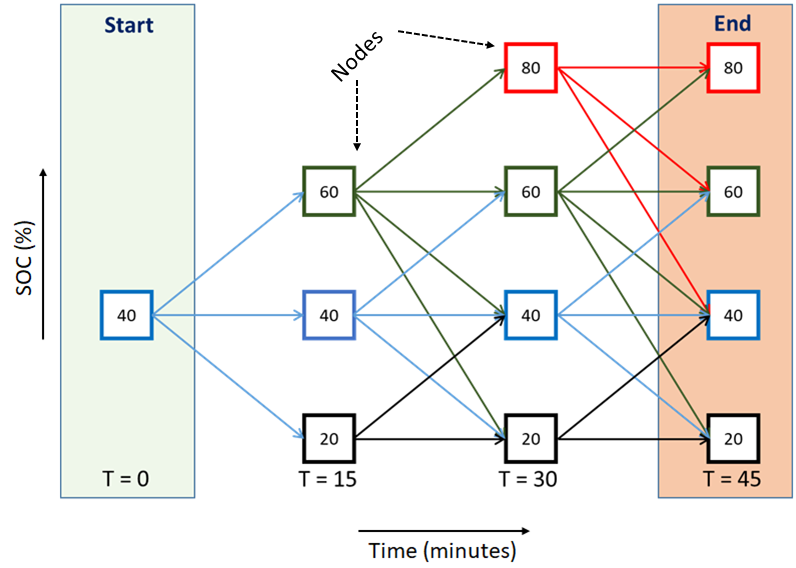
\includegraphics[width = \linewidth]{figs/F1_1_Dis.png}
    \caption{Discretizing solution space}
    \label{fig:F1_Dis}
\end{figure}
The horizontal axis of the figure represents time, and the vertical axis represents discrete steps in the state of charge (SOC) of the energy storage. In this simple example scenario, it is assumed that the algorithm recalculates the solution every 15 minutes (control horizon) based on available data. The SOC of the energy storage system (ESS) is discretized in steps of 20\%, and the SOC is limited between 80\% and 20\%. It is also assumed that the ESS can discharge a maximum of 40\% of its maximum SOC and charge a maximum of 20\% of its SOC in a 15 minute time step. These values are chosen arbitrarily in this simple example scenario to explain the problem. Taking these features into consideration, a directed graph is constructed looking ahead three time steps into the future. The square boxes represent nodes on the graph. The numbers inside the boxes represent the SOC of the ESS at that node. The arrows from the boxes represent all the possible states the ESS can be in the next time step according to the constraints of the system. The arrows are treated as edges of the graph. In this case, the edges are unidirectional. The goal is to find the most cost efficient path to reach T = 45 minute. Although in this example the algorithm considers T = 45 as the final stage, in actual application the final stage can be determined based on the actual use case.







%\begin{enumerate}
\item \textbf{Set goal node:} Set the current goal node as the first component of the predefined list of end nodes. 
%2
\item \textbf{Create open list from start node:} Expand the start node and create an open list with all the child nodes of the start node. The open list sorts it's members in a priority queue based on the cost. The the start node is added to the closed list.
%3
\item \textbf{Select and expand best node from open list:} The node with the lowest cost is selected from the nodes within the open list. The Selected node is expanded and the children of the selected node is added to the open list. The expanded node is then added to the closed list.
%4
\item \textbf{Repeat 3 until goal node is reached}
%5
\item \textbf{Construct shortest path to goal node}: After reaching the goal node the shortest path to the goal is constructed from the closed list by retracing the parent nodes from the goal node to the start node.
%6
\item \textbf{Calculate and record total cost:} The total cost for the shortest path is calculated and the path is recorded with the total cost in a list named \textit{path list}.
%7
\item \textbf{Set new goal}: The open and closed list are cleared. The next component in the list of end nodes is selected as the goal node.
%8
\item \textbf{Repeat 2-7 for all components of the end nodes list}
%9
\item \textbf{Select the path with the lowest cost in the path list as the optimum path.}
\end{enumerate}




\bibliographystyle{IEEEtran}
\bibliography{mybib.bib}

\ifCLASSOPTIONcaptionsoff
  \newpage
\fi

\end{document}


